\documentclass[journal,12pt,twocolumn]{IEEEtran}

\usepackage{setspace}
\usepackage{gensymb}

\singlespacing


\usepackage[cmex10]{amsmath}

\usepackage{amsthm}

\usepackage{mathrsfs}
\usepackage{txfonts}
\usepackage{stfloats}
\usepackage{bm}
\usepackage{cite}
\usepackage{cases}
\usepackage{subfig}

\usepackage{longtable}
\usepackage{multirow}

\usepackage{enumitem}
\usepackage{mathtools}
\usepackage{steinmetz}
\usepackage{tikz}
\usepackage{circuitikz}
\usepackage{verbatim}
\usepackage{tfrupee}
\usepackage[breaklinks=true]{hyperref}
\usepackage{graphicx}
\usepackage{tkz-euclide}
\usepackage{float}

\usetikzlibrary{calc,math}
\usepackage{listings}
    \usepackage{color}                                            %%
    \usepackage{array}                                            %%
    \usepackage{longtable}                                        %%
    \usepackage{calc}                                             %%
    \usepackage{multirow}                                         %%
    \usepackage{hhline}                                           %%
    \usepackage{ifthen}                                           %%
    \usepackage{lscape}     
\usepackage{multicol}
\usepackage{chngcntr}

\DeclareMathOperator*{\Res}{Res}

\renewcommand\thesection{\arabic{section}}
\renewcommand\thesubsection{\thesection.\arabic{subsection}}
\renewcommand\thesubsubsection{\thesubsection.\arabic{subsubsection}}

\renewcommand\thesectiondis{\arabic{section}}
\renewcommand\thesubsectiondis{\thesectiondis.\arabic{subsection}}
\renewcommand\thesubsubsectiondis{\thesubsectiondis.\arabic{subsubsection}}


\hyphenation{op-tical net-works semi-conduc-tor}
\def\inputGnumericTable{}                                 %%

\lstset{
%language=C,
frame=single, 
breaklines=true,
columns=fullflexible
}
\begin{document}
\newtheorem{theorem}{Theorem}[section]
\newtheorem{problem}{Problem}
\newtheorem{proposition}{Proposition}[section]
\newtheorem{lemma}{Lemma}[section]
\newtheorem{corollary}[theorem]{Corollary}
\newtheorem{example}{Example}[section]
\newtheorem{definition}[problem]{Definition}

\newcommand{\BEQA}{\begin{eqnarray}}
\newcommand{\EEQA}{\end{eqnarray}}
\newcommand{\define}{\stackrel{\triangle}{=}}
\bibliographystyle{IEEEtran}
\providecommand{\mbf}{\mathbf}
\providecommand{\pr}[1]{\ensuremath{\Pr\left(#1\right)}}
\providecommand{\qfunc}[1]{\ensuremath{Q\left(#1\right)}}
\providecommand{\sbrak}[1]{\ensuremath{{}\left[#1\right]}}
\providecommand{\lsbrak}[1]{\ensuremath{{}\left[#1\right.}}
\providecommand{\rsbrak}[1]{\ensuremath{{}\left.#1\right]}}
\providecommand{\brak}[1]{\ensuremath{\left(#1\right)}}
\providecommand{\lbrak}[1]{\ensuremath{\left(#1\right.}}
\providecommand{\rbrak}[1]{\ensuremath{\left.#1\right)}}
\providecommand{\cbrak}[1]{\ensuremath{\left\{#1\right\}}}
\providecommand{\lcbrak}[1]{\ensuremath{\left\{#1\right.}}
\providecommand{\rcbrak}[1]{\ensuremath{\left.#1\right\}}}
\theoremstyle{remark}
\newtheorem{rem}{Remark}
\newcommand{\sgn}{\mathop{\mathrm{sgn}}}
\providecommand{\abs}[1]{\vert#1\vert}
\providecommand{\res}[1]{\Res\displaylimits_{#1}} 
\providecommand{\norm}[1]{\lVert#1\rVert}
%\providecommand{\norm}[1]{\lVert#1\rVert}
\providecommand{\mtx}[1]{\mathbf{#1}}
\providecommand{\mean}[1]{E[ #1 ]}
\providecommand{\fourier}{\overset{\mathcal{F}}{ \rightleftharpoons}}
%\providecommand{\hilbert}{\overset{\mathcal{H}}{ \rightleftharpoons}}
\providecommand{\system}{\overset{\mathcal{H}}{ \longleftrightarrow}}
	%\newcommand{\solution}[2]{\textbf{Solution:}{#1}}
\newcommand{\solution}{\noindent \textbf{Solution: }}
\newcommand{\cosec}{\,\text{cosec}\,}
\providecommand{\dec}[2]{\ensuremath{\overset{#1}{\underset{#2}{\gtrless}}}}
\newcommand{\myvec}[1]{\ensuremath{\begin{pmatrix}#1\end{pmatrix}}}
\newcommand{\mydet}[1]{\ensuremath{\begin{vmatrix}#1\end{vmatrix}}}
\numberwithin{equation}{subsection}
\makeatletter
\makeatother
\let\StandardTheFigure\thefigure
\let\vec\mathbf
\renewcommand{\thefigure}{\theproblem}
\def\putbox#1#2#3{\makebox[0in][l]{\makebox[#1][l]{}\raisebox{\baselineskip}[0in][0in]{\raisebox{#2}[0in][0in]{#3}}}}
     \def\rightbox#1{\makebox[0in][r]{#1}}
     \def\centbox#1{\makebox[0in]{#1}}
     \def\topbox#1{\raisebox{-\baselineskip}[0in][0in]{#1}}
     \def\midbox#1{\raisebox{-0.5\baselineskip}[0in][0in]{#1}}
\vspace{3cm}
\title{QUIZ 2}
\author{Vaibhav Chhabra\\ AI20BTECH11022}
\maketitle
\newpage
\bigskip
\renewcommand{\thefigure}{\theenumi}
\renewcommand{\thetable}{\theenumi}
Download all latex-tikz codes from 
%
\begin{lstlisting}
    https://github.com/vaibhavchhabra25/EE3900-course/blob/main/QUIZ-2/main.tex
\end{lstlisting}
%
\section{Problem}
(3.8(b))
The system function of a casual linear time-invariant system is
\begin{align}
    H(z)=\dfrac{1-z^{-1}}{1+\frac{3}{4}z^{-1}}
\end{align}
The input to this system is 
\begin{align}
    x[n]=\left(\frac{1}{3}\right)^n u[n] + u[-n-1]
\end{align}
Find the output y[n].
\section{Solution}
The $\mathcal{Z}$ transform of x[n] is given by
\begin{align}
    X(z)&=\mathcal{Z}(x[n])\\
    &= \sum_{-\infty}^\infty (z^{-1})^n(x[n])\\
    &= \sum_{-\infty}^\infty (z^{-1})^n \left(\frac{1}{3}\right)^n u[n]+\sum_{-\infty}^\infty (z^{-1})^n u[-n-1]\\
    &= \sum_{0}^\infty \left(\frac{1}{3}z^{-1}\right)^n + \sum_{-\infty}^{-1} (z^{-1})^n\\
    &= \sum_{0}^\infty \left(\frac{1}{3}z^{-1}\right)^n + \sum_1^{\infty}z^n\\
    &= \dfrac{1}{1-\frac{1}{3}z^{-1}}-\dfrac{1}{1-z^{-1}}\\
    &= \dfrac{-\frac{2}{3}z^{-1}}{(1-\frac{1}{3}z^{-1})(1-z^{-1})}
\end{align}
where ROC of $X(z)$ is $\frac{1}{3}<|z|<1$.\\
Now, using convolution theorem, since
\begin{align}
    y[n]=h[n]*x[n]
\end{align}
we can write
\begin{align}
    Y(z)&= H(z)X(z)\\
    &= \left(\dfrac{1-z^{-1}}{1+\frac{3}{4}z^{-1}}\right)\dfrac{-\frac{2}{3}z^{-1}}{(1-\frac{1}{3}z^{-1})(1-z^{-1})}\\
    &= \dfrac{-\frac{2}{3}z^{-1}}{(1-\frac{1}{3}z^{-1})(1+\frac{3}{4}z^{-1})}\\
    &= \frac{24}{39}\left(\dfrac{1}{1+\frac{3}{4}z^{-1}}-\dfrac{1}{1-\frac{1}{3}z^{-1}}\right)\\
    &= \frac{24}{39}\left(\sum_{-\infty}^\infty \left(-\frac{3}{4}z^{-1}\right)^n u[n]-\sum_{-\infty}^\infty \left(\frac{1}{3}z^{-1}\right)^n u[n]\right)
\end{align}
The output signal y[n] is the inverse $\mathcal{Z}$ transform of $Y(z)$.
So,
\begin{align}
    y[n] = \frac{24}{39}\left(\left(\frac{-3}{4}\right)^n u[n] - \left(\frac{1}{3}\right)^n u[n]\right)\\
    y[n] = \frac{24}{39}\left(\left(\frac{-3}{4}\right)^n-\left(\frac{1}{3}\right)^n\right)u[n]
\end{align}
% \begin{figure}[!ht]
%     \centering
%     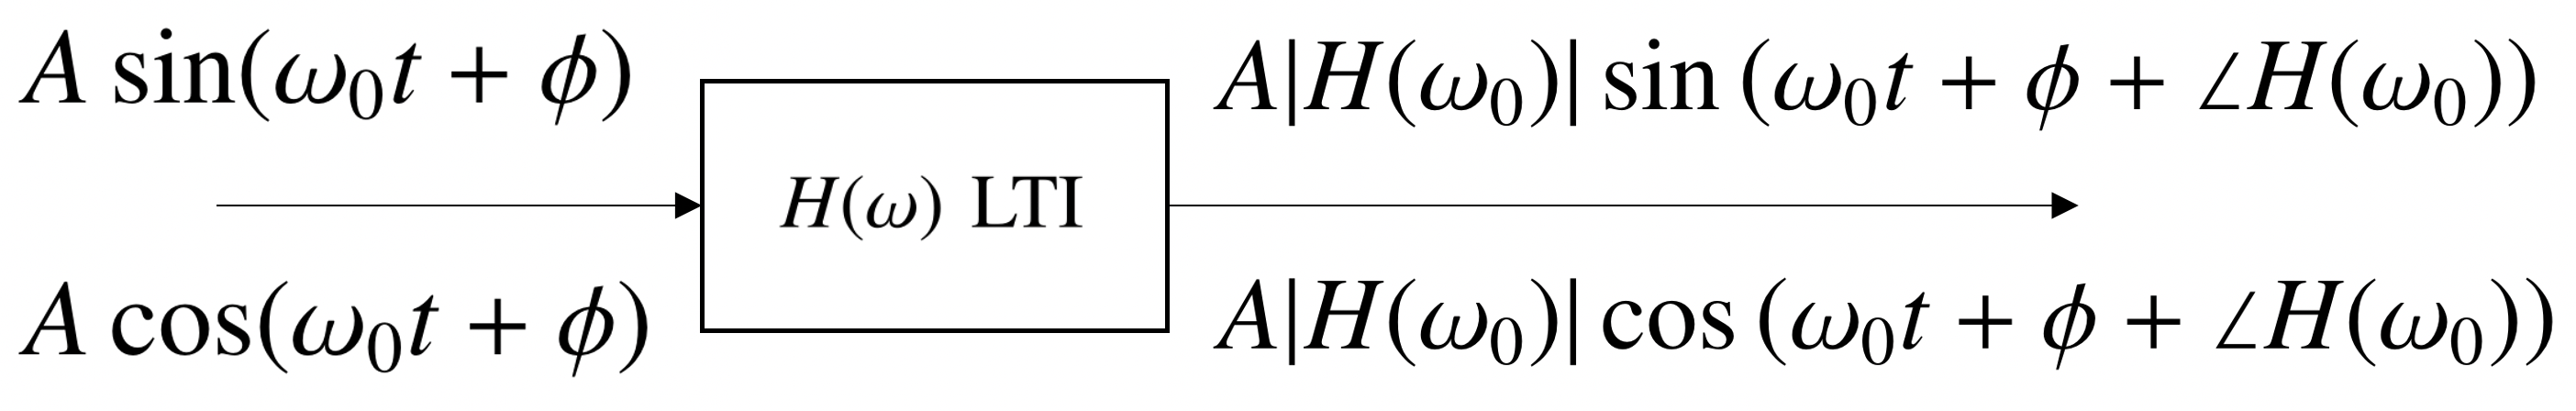
\includegraphics[width=\columnwidth]{figure.png}
%     \caption{ Plot for $x[n] = e^{j(2\pi n/5)}$ }
% \end{figure}
\end{document}
